\chapter{Gestión del proyecto} \label{chap:Gestion}
\chapterimage{figuras/ImagenesPortada/PortadaPlanificacion.jpg}
\hrule
\vspace{3mm}

En este capítulo se describe la gestión del proyecto: ciclo de vida, planificación y presupuesto, tanto del material utilizado como del coste que tendría el material para construir un prototipo funcional tal y como se ha diseñado.

\section{Ciclo de vida}

El proyecto, desde sus inicios ha ido pasando por una serie de fases que no siempre se han mantenido secuenciales. En la construcción de un brazo robótico se pueden separar diferentes etapas, que a grandes rasgos cubren todos los aspectos del diseño. Se puede ver un diagrama con las diferentes etapas en la figura \ref{fig:Gestion:fases_proyecto}, que se detallan a continuación.
\\

\begin{figure}
	\centering
	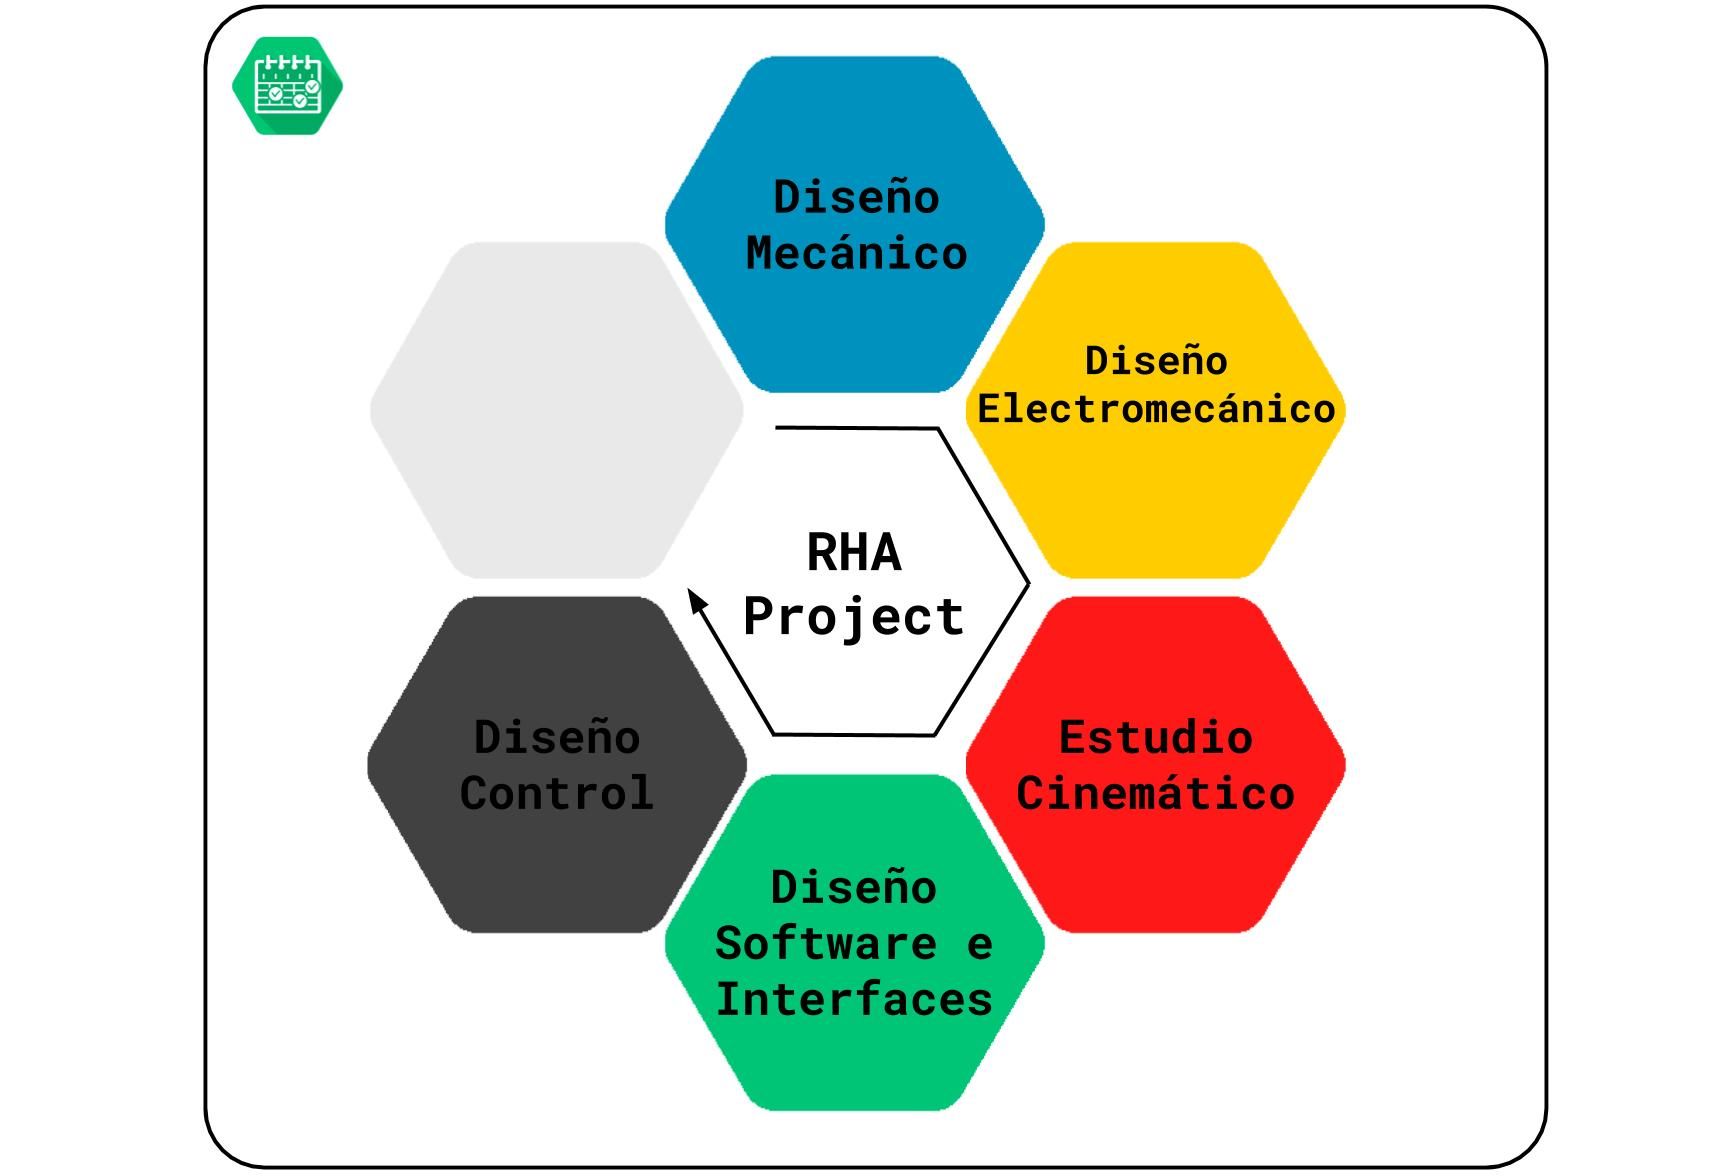
\includegraphics[width=1\textwidth]{figuras/Imagenes_Gestion/fases_proyecto.jpg}
	\caption{Diagrama con las diferentes fases del proyecto}
	\label{fig:Gestion:fases_proyecto}
	\immagesource{Autor}
\end{figure}


El primer paso para siempre pasa por el diseño del soporte físico del prototipo. Esta fase incluye una etapa de aprendizaje de las tecnologías a utilizar (impresión 3D y corte láser) así como el estudio de diferentes opciones y el desarrollo iterativo a través de las diferentes versiones. Las etapas finales del desarrollo mecánico o físico del proyecto se funden con las siguientes etapas, que implican adaptar parte de la estructura para incluir, de forma satisfactoria, el resto de aspectos constructivos o de control.
\\

Otra fase importante pasa por la elección del material electromecánico. Este material, sensores y actuadores, y su integración en el brazo robótico influye de forma notable en el diseño del propio brazo robótico. Es necesario tener definidos estos componentes antes de continuar con posteriores desarrollos para evitar inconsistencias con el diseño. En esta etapa será imprescindible comprobar que los sensores elegidos cubren el rango necesario, una vez integrados; de igual manera los actuadores deben ser capaces de realizar las operaciones tal y como se espera. Estas comprobaciones pueden implicar cambios en el diseño mecánico o en los elementos elegidos.
\\

Una vez se tiene el soporte físico completo, es decir, el esqueleto del brazo robótico, se puede pasar a la siguiente fase: el estudio matemático del mismo. Se entiende que llegados a esta fase los cambios que puede sufrir ls componentes mecánicos y electrónicos del prototipo no afectarán notablemente a las relaciones matemáticas del brazo (cinemática y dinámica) así como de los sensores.
\\

En este caso concreto, a continuación o incluso paralelamente al estudio matemático se comienza con la implementación del software. Es necesario generar un marco que permita controlar el brazo, aun de forma rudimentaria. Esta fase implica definir la estructura del software, la gestión interna de la información así como los componentes principales (a falta de las modificaciones pertinentes del control). Concretamente es de especial interés definir como se manejan los servos (protocolo de comunicación) y ciclos de funcionamiento entre los diferentes componentes. Una vez se tiene un marco lo suficientemente maduro (con la verificación y testing correspondiente de cada componente) se puede introducir la siguiente fase.
\\

Teniendo un sistema básico de software es imprescindible para poder hacer un estudio dinámico y estático del sistema. Usando de apoyo el desarrollo de software actual se obtiene la información del brazo que propiciará el análisis y diseño del sistema de control correspondiente. Una vez se tiene diseñado el control se procede a su implementación software.
\\

En cada etapa se debe ir comprobando el funcionamiento de conjunto según se acumulan funcionalidades. De esta forma, la verificación del funcionamiento como conjunto del brazo, una vez finalizado el ciclo, se vuelve más sencilla. 
\\

La figura \ref{fig:Gestion:fases_proyecto} representa estas fases a modo de ciclo. Como en todo proyecto de prototipado, una vez finalizada la primera etapa, y con un prototipo funcional, se han de tomar las decisiones pertinentes que, afectando a todas las etapas, permitan evolucionar a través de un nuevo ciclo el prototipo a una segunda versión. De esta manera el prototipo diseñado pasa por diferentes ciclos hasta que es completamente apto para comercializarse como producto.

\section{Planificación} \label{gestion:planificacion}

El ciclo de vida que se ha explicado en el apartado anterior puede desglosarse en detalle en la figura \ref{fig:Gestion:gantt_tareas}, donde se muestra un diagrama de Gantt con las diferentes actividades implicadas en el desarrollo del proyecto.
\\

El diagrama muestra una evolución temporal de los diferentes pasos seguidos en la ejecución y construcción del brazo robótico de forma que se puede observar, semana a semana, el tiempo dedicado a cada actividad.
\begin{landscape}
   	\begin{figure}[H]
   		\centering
   		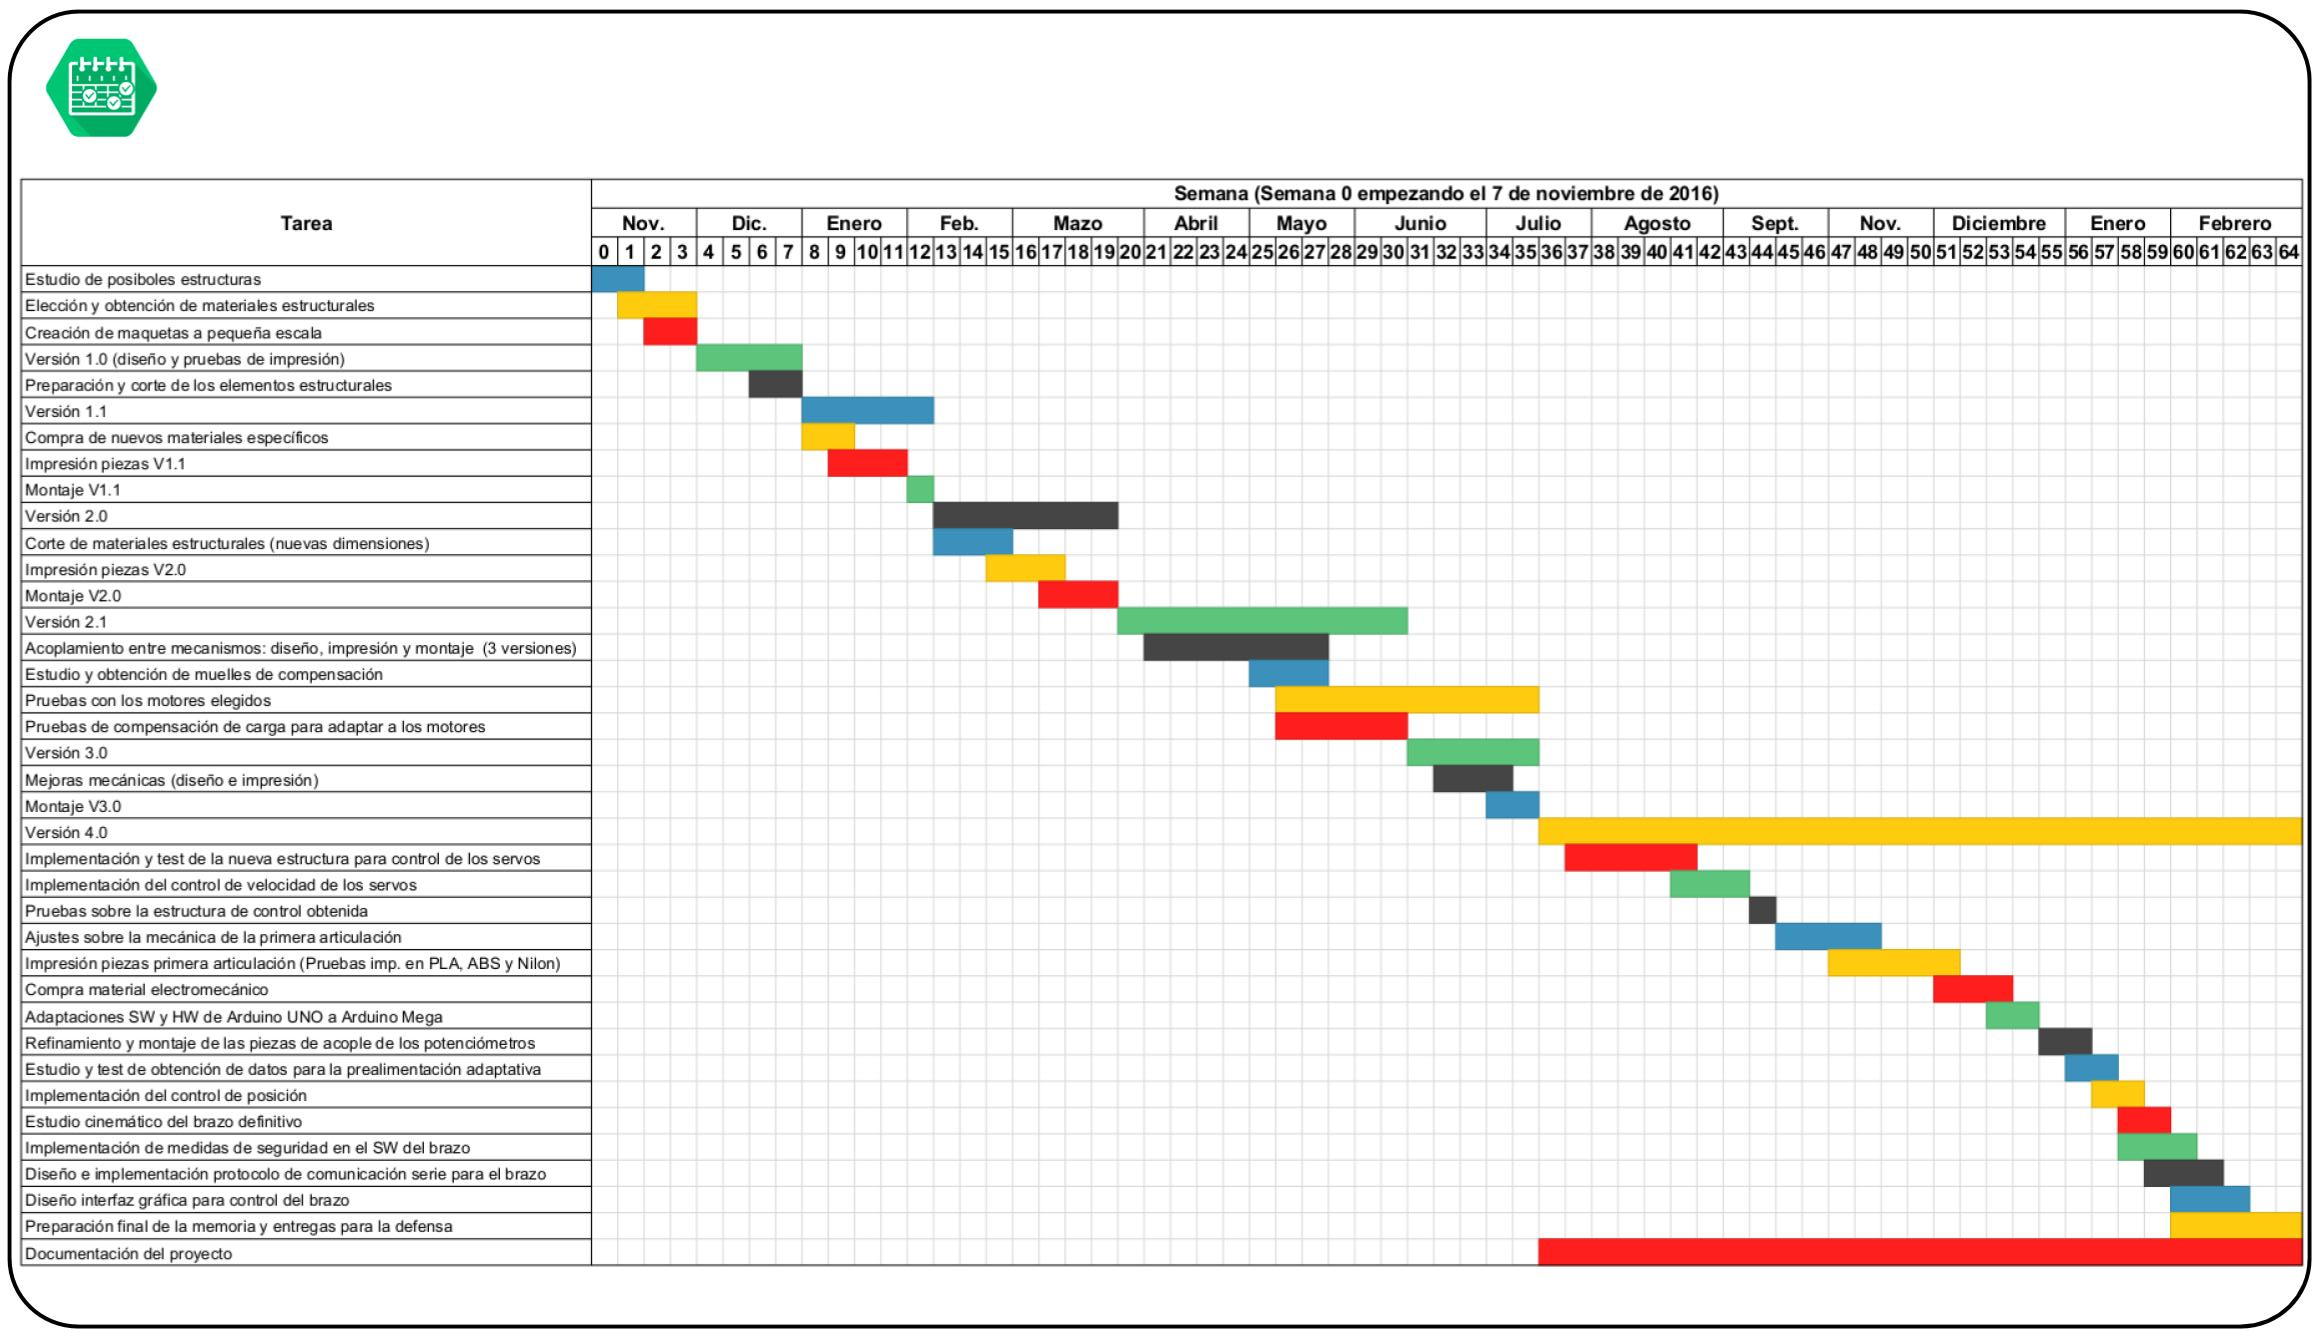
\includegraphics[width=1.6\textwidth]{figuras/Imagenes_Gestion/organizacion_gantt.jpg}
   		\caption{Diagrama de Gantt con la distribución temporal de tareas}
   		\label{fig:Gestion:gantt_tareas}
   		\immagesource{Autor}
   	\end{figure}
\end{landscape}

\section{Presupuesto}

    Se puede ver el coste de los materiales en la tabla \ref{tab:presupuesto} así como el presupuesto estimado para la construcción del prototipo. Se debe tener en cuenta que para la estimación del precio total se han tomado los precios resultantes de la compra de unidades sueltas a través de los distribuidores oficiales para cada caso. De igual manera, parte de los materiales que se presentan no son consumidos en su totalidad  en la realización de un solo montaje, si no que valdrían para varios. 
    \\
    
    El presupuesto que se muestra se puede tomar como referencia del coste máximo que conllevaría la construcción, a pequeña escala, del brazo robótico diseñado.

    \renewcommand{\thempfootnote}{\arabic{mpfootnote}}

    \begin{table}[H]
    \caption{Costes del proyecto}
    \label{tab:presupuesto}
    \begin{center}
    \begin{minipage}{\textwidth}
    \begin{tabular}{ |c|c|c|c|c| }
    \hline
    \textbf{Artículo} & \textbf{Referencia} & \textbf{Coste Unitario} \footnote{En los casos en qué ha sido necesario se ha aplicado el cambio a Euros oficial propuesto por \cite{bancoEspana} en el día en que se han consultado los precios} & \textbf{Cantidad} & \textbf{Total} \\
    \hline
    \hline
    %Arduino Uno & GBX00066 & 17.00 \euro\footnote{Precios consultados en \cite{arduinoStore} a 07 de Septiembre 2017.} & 1 & 17.00 \euro\\
    Arduino Mega & A000067 & 35.00 \euro\footnote{Precios consultados en \cite{arduinoStore} a 19 de Febrero 2018.} & 1 & 35.00 \euro\\
    Cytron G15 Cube Servo & G15 & 23.23 \euro\footnote{Precios consultados en \cite{cytronStore} a 07 de Septiembre 2017.} & 3 & 69.69\euro \\
    Cytron G15 Shield & SHIELD-G15 & 6.64 \euro\footnote{Precio consultados en \cite{cytronStore} a 07 de Septiembre 2017.} & 1 & 6.64 \euro\\
    \hline
    \hline
    Potenciómetro Serie TW & 502-8621 &  9.29 \euro\footnote{Precio consultados en \cite{rsStore} a 07 de Septiembre 2017.} & 2 & 18.58\euro \\
    Fuente de alimentación & S-120-12  &  12.05 \euro\footnote{Precio consultados en \cite{aliexpres} a 19 de Febrero 2018.} & 1 & 12.05\euro \\
    \hline
    \hline
    Perfiles Aluminio sección cuadrada & 304-7894 & 5.626 \euro\footnote{Precio consultados en \cite{rsStore} a 07 de Septiembre 2017.} & 5 & 28.13 \euro \\
    Rodamiento 13x4 & 618-9890 & 1.83\euro\footnote{Precio consultados en \cite{rsStore} a 20 de Enero 2018.} & 14 & 25.62 \euro \\
    Rodamiento 10x3 & 618-9856 & 2.02\euro\footnote{Precio consultados en \cite{rsStore}S a 20 de Enero 2018.} & 2 & 4.04 \euro \\
    Rodamiento Axial & 286-8549 & 23.57\euro\footnote{Precio consultados en \cite{rsStore}S a 19 de Febrero 2018.} & 1 & 23.57\euro \\
    Poleas acetal 10x3 & 352-0636 & 2.30\euro\footnote{Precio consultados en \cite{rsStore}S a 19 de Febrero 2018.} & 2 & 4.60\euro \\
    Hilo Kevlar (100ft 300lb) &-& 9.99 \euro\footnote{Precio consultados en \cite{emmakites} a 07 de Septiembre 2017.} & 1 & 9.99 \euro \\
    GM Series Plastic Wheel & GMPW & 2.70 \euro\footnote{Precio consultados en \cite{solarBotics} a 11 de Septiembre 2017.} & 1 & 2.70 \euro \\
    Parasol Hormigón 24kg & 15710142 & 27.95 \euro\footnote{Precio consultados en \cite{leroyMerlin} a 11 de Septiembre 2017.} & 1 & 27.95 \euro \\
    Muelle Tracción (1.8x200mm, 17kg) &  18613553 & 3.70 \euro\footnote{Precio consultados en \cite{leroyMerlin} a 11 de Septiembre 2017.} & 2 & 7.40 \euro \\
    Tornillería variada (ver tabla \ref{tab:tornilleria}) &  - & -  & - & - \\
    \hline
    \hline
    PLA filamento (1.75mm, 1kg) &  - & 19.90 \euro\footnote{Precio consultados en \cite{bq} a 11 de Septiembre 2017.} & \completar & n.00 \euro \\
    \hline
    \hline
    & & & Total: & 275.96 \euro \\
    \hline
    \end{tabular}
    \end{minipage}
    \end{center}
    \end{table}
    
    \completarCon{Ejes de acero de 4 y 3mm}
    
    La tornillería utilizada venía como parte de una caja con múltiples componentes. El precio del total no resulta representativo, es por eso que en la tabla \ref{tab:tornilleria} se muestran las necesidades de tornillería del prototipo sin incluir el precio de los mismos.
    
    \begin{table}[H]
    	\caption{Tornillería requerida}
    	\label{tab:tornilleria}
    	\begin{center}
    		\begin{tabular}{ |c|c|c| }
   			\hline
    		Modelo & Cantidad \\
    		\hline
    		Tuercas M4 & 26 \\
    		Tuercas M3 & 17 \\
    		Tornillos M3x10 & 15 \\
    		Tornillos M3x25 & 2 \\
    		Tornillos M4x10 & 4 \\
    		Tornillos M4x12 & 2 \\
    		Tornillos M4x20 & 18 \\
    		\hline
    	\end{tabular}
	\end{center}
	\end{table}

